% =============================================================================
% CAPÍTULO 7 — volta 1, a última forma: a dependência que a margem não vê.
%
% O fracasso que o abre, com número na mão: dois mercados protegidos cada um no seu corte de
% 5% rompem juntos 7,17 vezes mais do que a independência prevê, e nenhum instrumento dos
% capítulos 4 e 5 pode ver isso — a informação não está em nenhuma das duas séries.
%
% A prova de cegueira é medida: deslocando só o pareamento do segundo mercado, a primeira
% perna rompe os MESMOS 315 dias e a razão contra a independência cai de 7,17 para 1,43.
%
% Medição: lab/experimentos/E05_dependencia.ipynb e lab/experimentos/E46_identificacao.ipynb. Figuras: figuras/E05_dependencia_* e figuras/E46_identificacao_*.
% =============================================================================

\chapter{O dia em que tudo cai junto}
\label{cap:dependencia}

\section{O que a margem não vê}

Os três capítulos anteriores vigiaram uma série por vez: o corte, o vigia, a célula do
calendário. Todos eles leem uma margem, e aqui se trata de duas ao mesmo tempo. Ele começa por uma
tentativa que qualquer mesa faz: proteger cada mercado no seu próprio corte de
\numPromessaPct\%, e supor que a proteção dos dois é a soma das duas.

O par é o índice americano e o brasileiro: \numDependenciaDias{} dias em que os dois têm
corte, dos \numPedacoDiasComuns{} em que os dois existiram, um quarto de século de mercado. Cada um rompeu o seu próprio corte na mesma taxa: \numDependenciaTaxaAPct\% dos dias de um
lado, \numDependenciaTaxaBPct\% do outro, ou \numDependenciaRompeA{} rompimentos e
\numDependenciaRompeB{} --- a promessa do corte sendo cumprida duas vezes.

Agora a conta que interessa: se os dois mercados fossem independentes, os dias em que os dois
rompem seriam o produto das duas taxas, e ao longo de \numDependenciaDias{} dias isso daria
\numDependenciaEsperadoDias{} dias. Aconteceram \numDependenciaJuntos: \numDependenciaJuntosPct\%
dos dias, contra os \numDependenciaEsperadoPct\% que a independência preveria. A razão entre o que se mediu e o que a independência previa é de \numDependenciaExcesso{} vezes.

Dito pela outra ponta, que é como quem carrega a posição sente: dos \numDependenciaRompeA{}
rompimentos do primeiro mercado, \numDependenciaAcompanhadosPct\% vieram acompanhados por um
rompimento do segundo. Somando as duas proteções, esperar-se-ia
% aterramento: dependencia
\numDependenciaAcompanhadosIndependentePct\%.
A \textbf{dependência} entre duas séries é o quanto saber de uma muda o que se espera da outra.
O caso extremo é a independência, em que saber de uma não muda nada: a chance de as duas
romperem no mesmo dia passa a ser o produto das duas chances. Essa fração é a dependência de
cauda, e estimá-la de uma amostra finita tem viés próprio \cite{garcin2026nonparametric}.

\section{A conta que a soma faz}

Vale escrever por que a soma erra, porque o erro não é de aritmética. Se as duas pernas fossem
independentes, a chance de as duas romperem no mesmo dia seria o produto das duas: é o que faz
a soma das proteções ser, ao mesmo tempo, correta e inútil. O produto supõe que saber de uma
perna não diga nada sobre a outra, e é exatamente isso que um dia ruim desmente.

\begin{proposicao}[o teto do par]\label{prop:teto-do-par}
Se cada perna rompe o próprio corte com probabilidade $p$, a chance de as duas romperem no mesmo
dia não passa de $p$, por mais forte que seja a dependência entre elas. A independência preveria
$p^{2}$, de modo que o par pode entregar até $1/p$ vezes o que a soma prevê.
\end{proposicao}

\begin{proof}
O acontecimento \emph{as duas rompem} está contido em \emph{a primeira rompe}, e a probabilidade
de um acontecimento não passa da probabilidade do que o contém: a chance conjunta não passa de
$p$. A independência é o outro extremo, com $p^{2}$, e a razão entre os dois extremos é $1/p$ ---
vinte no corte de \numPromessaPct\%.
\end{proof}

A medida que este capítulo usa não é a correlação, e a escolha é deliberada. Correlação é uma
média do miolo: ela resume os dias comuns, que são a maioria, e não tem motivo nenhum para
acertar na cauda, que é onde a conta é paga. O que se conta aqui é mais cru e mais direto:
quantos dias as duas romperam o próprio corte, contra quantos dias a independência preveria.
Nenhuma forma de dependência é suposta --- não há normalidade, não há cópula, não há parâmetro
---, só a contagem dos dias em que as duas séries existem\cite{pfister2018kernel,szekely2007measuring}.
% aterramento: copula
A \textbf{cópula}, que é a peça dispensada aqui, é a função que costura duas séries pela
dependência delas depois de cada uma ter sido posta na própria unidade: ela descreve a
junta inteira, e para isso tem de ser escolhida\cite{clemente2021calibrating} --- e escolher errado erra na cauda, que é onde a
conta é paga\cite{ansari2021sklar}.

A cota da \cref{prop:teto-do-par} diz quanto essa contagem pode andar: o par como veio entrega
\numDependenciaExcesso{} vezes o que a soma prevê, e o teto do corte de \numPromessaPct\% é de vinte
vezes.

\begin{figure}[htbp]
  \centering
  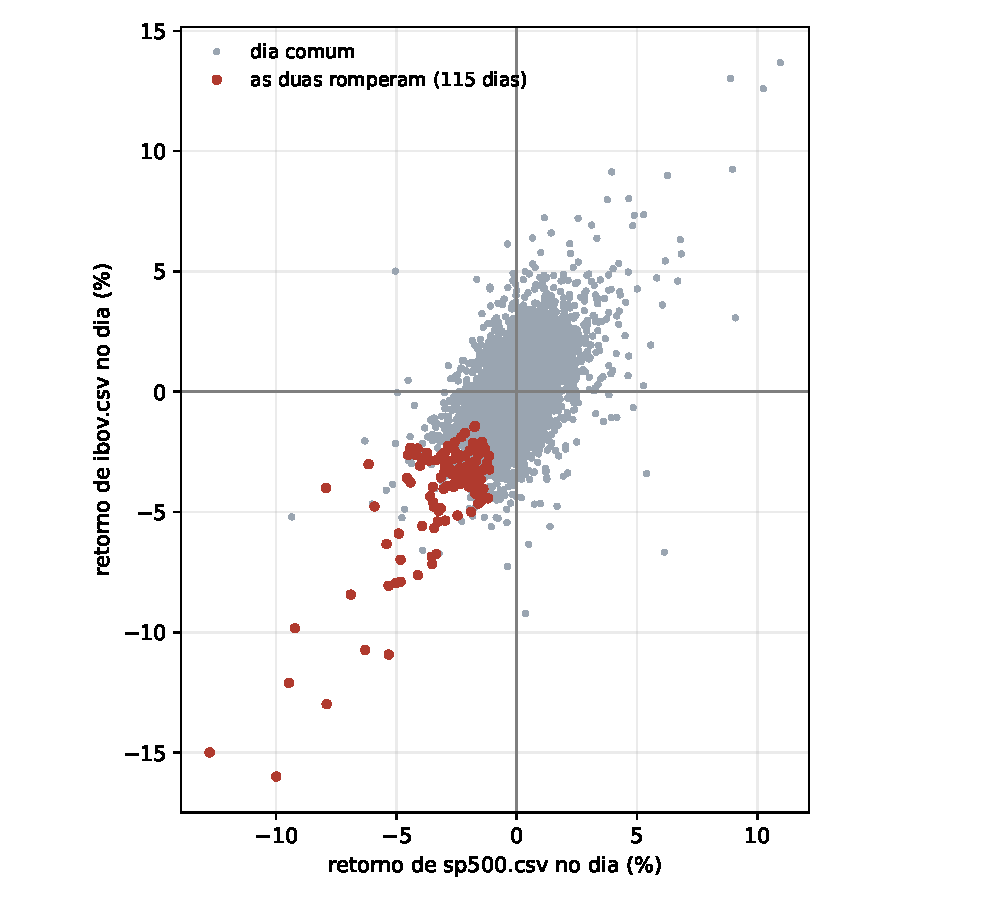
\includegraphics[width=0.82\linewidth]{figuras/E05_dependencia_1.pdf}
  \caption{Os dois mercados, dia a dia. Cada ponto é um dia, com o retorno de um no eixo
    horizontal e o do outro no vertical; as linhas em zero partem o plano em quadrantes. Os
    \numDependenciaJuntos{} dias em que as duas pernas romperam estão todos no quadrante de
    baixo à esquerda, e nenhum em qualquer outro lugar do plano.}
  \label{fig:nuvem}
\end{figure}

As duas retas do desenho marcam o zero de cada mercado, e o corte de cada dia fica bem mais fundo
que ele: o quadrante de baixo à esquerda é muito maior do que o punhado de pontos vermelhos que ele
contém. Quem passa o olho encontra ali todo dia de queda, e a figura marca outra coisa --- o dia em
que as duas pernas foram ao fundo juntas.

\section{A cópula que a contagem não escolhe}

A seção anterior dispensou a cópula com um argumento de gosto: se ela tem de ser escolhida,
escolher errado erra na cauda. Aqui o argumento deixa de ser de gosto e vira consequência de
teorema --- e a razão está na margem deste capítulo. A margem é de contagem: o dia rompe o corte
ou não rompe, e numa margem assim a probabilidade integral só visita três pontos, que são o zero,
o ponto em que ela salta e o um.

% aterramento: subcopula
Nessa grade, a junta inteira se decide em quatro cantos: os dois que cada perna assina sozinha, o
canto do um, e o canto de dia nenhum, que é o único que a contagem conjunta assina. O objeto que
carrega esse pouco sem inventar o resto é a \textbf{subcópula}: a cópula lida apenas no grade das
margens medidas. São \numFamiliaConjuntos{} dias em que as duas pernas romperam juntas, e é
\emph{tudo} o que a contagem conjunta diz.

% aterramento: familia-de-extensoes
% aterramento: conjunto-identificado
O teorema de Sklar garante que existe cópula casando as margens, e não garante que ela seja uma
só: o que a subcópula deixa em aberto é preenchido pelas \textbf{medidas duplamente estocásticas}
que a estendem, e delas há infinitas \cite{amo2012characterization}. É aqui que a escolha que a
seção anterior tratava como risco muda de estatuto. Com margem de contagem, escolher a cópula não
é uma decisão arriscada: é uma decisão que o dado não determina. Quem escolhe, escolhe sozinho. O \textbf{conjunto identificado} é o que sobra dessa conta:
a banda que a contagem admite e não fecha.

O instrumento constrói um subconjunto \emph{declarado} dessas extensões --- a gaussiana, uma t
para cada grau de liberdade e a mistura das duas bordas, em \numFamiliaMembros{} membros ---, e
cada membro tem a correlação resolvida por bisseção para casar a massa \emph{medida}, e não a
nominal. Todos casam: o resíduo máximo é de \numFamiliaResiduoMax. No corte deste capítulo os
cinco preveem a mesma taxa conjunta, e ela é a medida. A família está colada onde a contagem fala.

\begin{figure}[htbp]
  \centering
  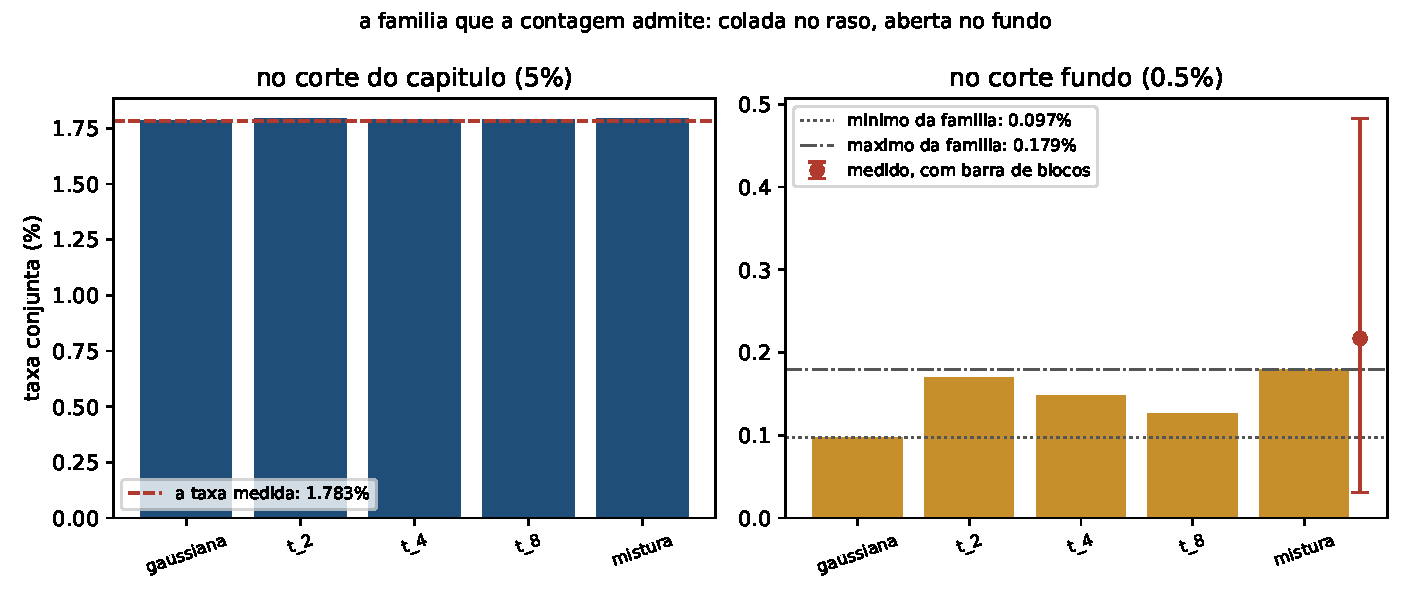
\includegraphics[width=\linewidth]{figuras/E46_identificacao_1.pdf}
  \caption{A taxa conjunta que cada membro da família prevê, no corte deste capítulo e no corte
    fundo. No painel da esquerda as cinco barras têm a mesma altura e a linha da taxa medida
    passa sobre elas; no da direita as mesmas barras se abrem, e o ponto medido vem com a barra de
    blocos.}
  \label{fig:familia}
\end{figure}

No corte fundo ela se abre --- e o dado fica do lado de fora. A \numFamiliaFundoPct\% da
distribuição, os cinco membros discordam entre \numFamiliaFundoMinPct\% e
\numFamiliaFundoMaxPct\% --- \numFamiliaFundoRazao{} vezes entre o mínimo e o máximo ---, e a
taxa medida naquele corte é \numFamiliaFundoMedidoPct\%, acima do máximo da família declarada. A
taxa medida entra na banda em \numFamiliaCortesDentro{} dos \numFamiliaCortes{} cortes medidos, e
a barra de blocos daquele corte é de \numFamiliaFundoBarraPct{} pontos percentuais: com
\numFamiliaConjuntos{} dias conjuntos, o corte fundo tem poucos dias, e a barra engole a
distância. O que fica dito é o que se pode dizer: a contagem deixa uma banda em aberto, e a
amostra não é grande o bastante para dizer onde o dado cai dentro dela.

\begin{figure}[htbp]
  \centering
  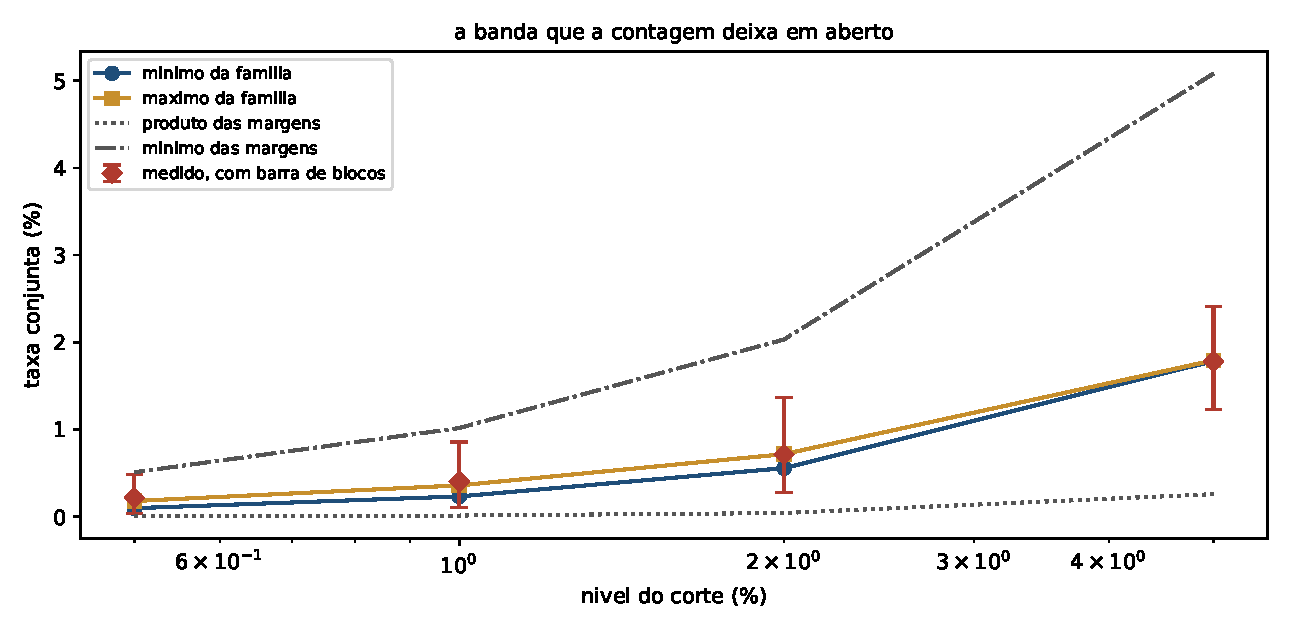
\includegraphics[width=\linewidth]{figuras/E46_identificacao_2.pdf}
  \caption{A banda que a contagem deixa em aberto, contra o nível do corte. As duas bordas da
    família se afastam quando o corte desce; os pontos medidos vêm com a barra de blocos, e as
    linhas pontilhadas são as bordas de Fréchet do par --- o produto das margens por baixo e o
    mínimo delas por cima.}
  \label{fig:banda}
\end{figure}

Falta o controle que separa a largura da banda do achar das duas pernas: um par
\emph{independente}, do mesmo tamanho e submetido à mesma rotina, tem razão de
\numFamiliaControleRazao{} no mesmo corte, contra \numFamiliaFundoRazao{} do par medido. A banda
não é do achar das pernas, e no par sem dependência nenhuma ela é ainda mais larga: o que a
contagem deixa em aberto é grandeza da contagem.

\section{O par é que decide}

Falta a parte difícil, que é mostrar que nada disso está em nenhuma das duas séries. A
experiência é simples e é decisiva: desloque o segundo mercado em um dia, em três semanas, em
um ano, em dois anos. Cada perna continua com os seus próprios números, na sua própria ordem;
o que muda é o \emph{par} --- qual dia de um mercado encontra qual dia do outro.

\begin{table}[htbp]
  \centering
  \resizebox{\linewidth}{!}{%
\begin{tabular}{lrr}
    \hline
    o par & rompe o primeiro & contra a independência \\
    \hline
    o que o mundo fez & \numDependenciaRompeA & \numDependenciaExcesso \\
    um dia depois & \numDependenciaRompeA & \numDependenciaAtrasoUmDiaExcesso \\
    três semanas depois & \numDependenciaRompeA & \numDependenciaAtrasoVinteEUmDiasExcesso \\
    um ano depois & \numDependenciaRompeA & \numDependenciaAtrasoUmAnoExcesso \\
    dois anos depois & \numDependenciaRompeA & \numDependenciaAtrasoDoisAnosExcesso \\
    \hline
  \end{tabular}}
  \caption{A mesma série, com o par trocado. A coluna da esquerda é a que importa: a
    primeira perna rompe os mesmos \numDependenciaRompeA{} dias em todas as linhas, porque a
    série dela não foi tocada. O pareamento é a única coisa que mudou.}
  \label{tab:par}
\end{table}

A primeira coluna da tabela é a resposta inteira. A perna do primeiro mercado rompe os mesmos
\numDependenciaRompeA{} dias nas cinco linhas: a margem dela não se mexeu, e nenhum instrumento
que leia essa série --- nem a contagem do alarme, nem a célula do calendário --- pode
distinguir uma linha da outra, porque não há nada a distinguir. O que muda é só a conta
conjunta, que cai de \numDependenciaExcesso{} vezes a independência para
\numDependenciaAtrasoUmDiaExcesso{} com um único dia de deslocamento, e para perto de um quando
o atraso passa de três semanas.

Um dia de deslocamento já destrói quase tudo, e isso diz onde a dependência mora: no mesmo dia.
A correlação conta a mesma história por outro caminho --- \numDependenciaCorrelacao{} com o par
real, \numDependenciaAtrasoUmDiaCorrelacao{} com o par deslocado por um dia ---, e é útil aqui
só como conferência, porque ela é a média que o miolo vê e não a contagem que a cauda paga.

\section{O controle}

Antes de aceitar um número desses, vale olhar o que ele dá quando não há nada para medir. Dois
mundos sorteados independentes, com a mesma rotina de corte: as razões
\numDependenciaExcesso{}, \numDependenciaAtrasoUmDiaExcesso{} e companhia não significam nada se
a conta também der sete quando as duas séries não têm nada a ver uma com a outra.

Sorteamos duas séries independentes do tamanho do par real e medimos o mesmo número: \numDependenciaControleExcesso{} vezes a independência. É o que tem de dar: a medida vale um
quando não há dependência, e é contra esse um que as outras linhas se leem.

\section{O que a proteção individual não cobre}

Falta o preço, e ele é o que decide se o número interessa a quem carrega a posição. Montamos a
carteira de peso igual nas duas pernas e olhamos a perda média em dois conjuntos de dias: os
\numDependenciaJuntos{} em que as duas romperam, e os quatrocentos e dois em que só uma rompeu.

No dia em que as duas rompem, a carteira perde \numDependenciaPerdaJuntosPct\%; no dia em que só
uma rompe, perde \numDependenciaPerdaUmaPernaPct\%. A razão entre as duas perdas é de \numDependenciaPerdaRazao{} vezes, e o dia conjunto é mais fundo que o dia de uma perna só: é justamente aquele em que as duas proteções são chamadas ao mesmo tempo.

\begin{figure}[htbp]
  \centering
  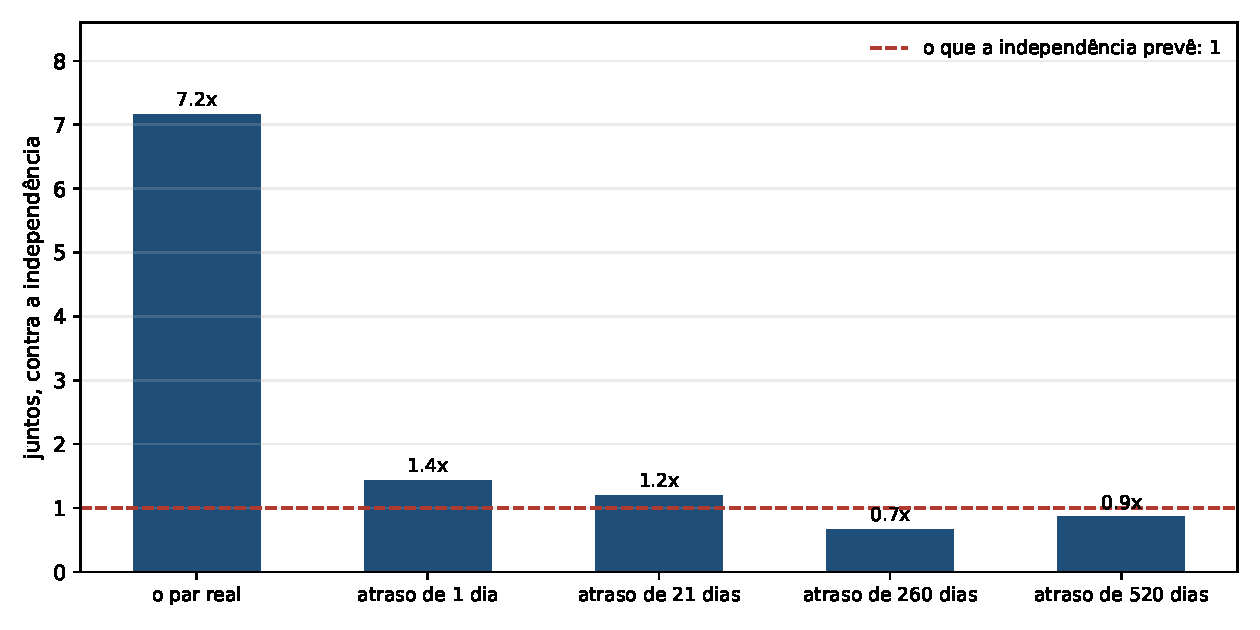
\includegraphics[width=\linewidth]{figuras/E05_dependencia_2.pdf}
  \caption{A barra da esquerda é o par como o mundo fez; as outras quatro são o mesmo par com o
    segundo mercado deslocado, e a linha tracejada é o que a independência prevê.
    Quase toda a dependência morre com um único dia de deslocamento.}
  \label{fig:par}
\end{figure}

\section{Quanto custa contar os pares}
% aterramento: concordancia
% aterramento: binomio
% aterramento: sigma-um
% aterramento: fracao-de-pares

O contador deste capítulo custa uma passada sobre os \numDependenciaDias{} dias, e responde olhando o
dia: rompeu ou não rompeu. A pergunta "os dois mercados andam juntos?" tem outra resposta possível, e
ela não olha o dia --- olha o \textbf{par} de dias: dois dias concordam quando os dois mercados andam
para o mesmo lado, e a medida é a fração de pares concordantes menos a de discordantes. Sobre os
mesmos \numDependenciaDias{} dias existem \numParesTotalMilhoes{} milhões de pares, e contar
todos eles é o gesto caro
que este pedaço cobra.

\begin{proposicao}[o preço de contar pares]\label{prop:preco-dos-pares}
Sorteie uma fração $\rho$ dos pares, com os dois dias de cada par escolhidos independentemente. A
concordância assim medida tem o mesmo valor esperado da que usa todos os pares, e desvio
$\sigma/\sqrt{\rho \binom{n}{2}}$ --- com $\sigma^2 = 1 - \tau^2$, a variância do kernel binário,
que é exata e não estimada. A barra do \emph{dado}, que não depende de quantos pares se conta, é
$\sqrt{(2(n-2)\sigma_1^2 + \sigma^2)/\binom{n}{2}}$, com $\sigma_1^2$ a covariância entre dois pares
que dividem um dia.
\end{proposicao}

\begin{proof}
Cada par de dias contribui com $+1$ ou $-1$, de modo que a variância do kernel é $1-\tau^2$ sem
estimativa nenhuma. Pares sorteados independentemente não têm covariância entre si --- a sobreposição
de dias que existe entre pares \emph{distintos} da população não entra nesta conta ---, e a média de
$\rho\binom{n}{2}$ deles tem o desvio da proposição. Para a segunda barra, a variância de uma
U-estatística de ordem dois com todos os pares é a de Hoeffding: $\binom{n}{2}$ no denominador, e no
numerador a covariância que os pares carregam por dividir dias entre si.
\end{proof}

A medição usa o par deste capítulo --- os mesmos \numDependenciaDias{} dias, o mesmo corte ---, e
sorteia \numParesMundos{} mundos por linha. A concordância exata é \numParesTau{}, e as barras vão em
milésimos, para os algarismos caberem na página.

\begin{table}[htbp]
  \centering
  \small
  \begin{tabular}{rrr}
    \hline
    pares usados & barra do sorteio & a lei prevê \\
    \hline
    todos & \numParesMedidoTodos & \numParesBarraTodos \\
    meio & \numParesMedidoMeio & \numParesBarraMeio \\
    um décimo & \numParesMedidoDecimo & \numParesBarraDecimo \\
    um centésimo (\numParesCentesimo) & \numParesMedidoCentesimo & \numParesBarraCentesimo \\
    \hline
  \end{tabular}
  \caption{A barra da concordância contra a fração dos pares que se conta, medida em
    \numParesMundos{} mundos e comparada com a lei.}
  \label{tab:pares}
\end{table}

A lei acerta em toda a extensão, e o número que decide não está na tabela: a barra do sorteio com um
centésimo dos pares é dez vezes a barra com todos eles, e mesmo assim vale \numParesCustoPct{} por
cento da variância que o mercado impõe sozinho --- que é a outra barra, a do dado, de
\numParesBarraDoDado{} milésimos. Quem conta pares nunca esteve limitado pelos pares.

\begin{figure}[htbp]
  \centering
  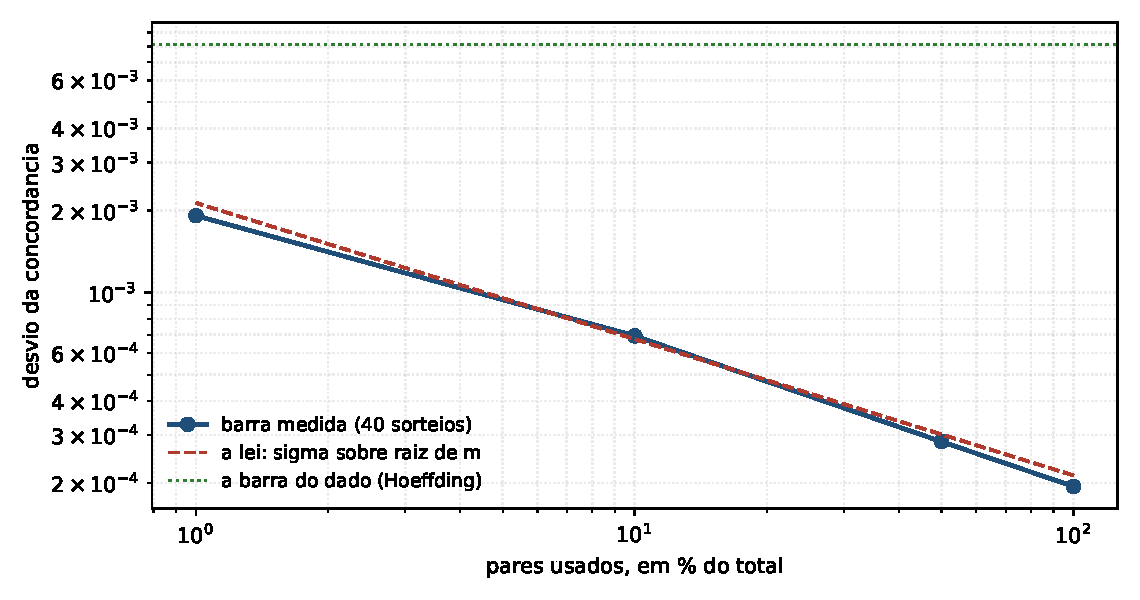
\includegraphics[width=\linewidth]{figuras/E30_pares_1.pdf}
  \caption{A barra do sorteio contra a fração dos pares que se conta, nas duas escalas logarítmicas,
    com a lei ao lado, e a barra do dado como linha no alto. A linha medida quase coincide com a lei
    em toda a extensão, e a linha do dado fica acima das duas: \textbf{o que a economia de pares
    custa é pequeno diante do que o mercado já cobra.}}
  \label{fig:pares}
\end{figure}

E a concordância exata não precisa de par nenhum. Ela sai de ordenar as duas séries --- o número de
pares concordantes é o de inversões de uma permutação, e inversões se contam sem enumerá-las ---, e o
caderno mede isso: \numParesTempoExato{} segundos para os dezenove milhões de pares. O que existe é o
número deles, e não a lista. Quando a medida não tem forma fechada, é o algoritmo que a põe em uso: a
distância de covariância olha toda a dependência sem supor forma nenhuma \cite{szekely2007measuring},
e o que a tornou prática foi a conta que evita as comparações duas a duas \cite{huo2016fast}. A
contagem com uma parte dos pares é a U-estatística incompleta de Blom \cite{blom1976some} --- e a
tabela acima é ela, medida.

Este número não substitui o do capítulo, e não é para substituir: um conta os dias em que as duas
pernas rompem, o outro mede o quanto os dois mercados andam juntos. O controle do capítulo vale para
os dois --- no par sorteado independente a concordância é \numParesControleTau{}.

\section{O que fica}

Fica um instrumento, e ele é pequeno o bastante para caber numa frase: \textbf{conte os dias em
que as duas coisas rompem, e compare com o que a independência preveria}. A razão entre os dois
não supõe forma nenhuma de dependência, não precisa de normalidade nem de cópula, e responde à
pergunta que a soma das proteções responde errado.

E fica o que este capítulo mostrou sobre os capítulos anteriores, que é mais desconfortável do
que o número. O vigia do alarme e a célula do calendário leem margens, e o pareamento não mora em margem alguma. Mudar o par deixa as duas séries idênticas a si mesmas e muda a conta. Não é que aqueles instrumentos sejam fracos --- é que a pergunta que este capítulo faz não
é uma pergunta sobre uma série.

O fracasso seguinte nasce do próprio número que ficou. \numDependenciaExcesso{} vezes a
independência é uma média sobre um quarto de século de pregões; ela diz que os dois caem juntos mais do que a
sorte explicaria, e não diz \emph{desde quando}. Existe um dia em que a dependência mudou --- em
que o par deixou de valer o que valia ---, e a mesma estatística que responde "que conjunto ainda
vale" responde "em que instante ele deixou de valer", lida ao contrário. Separar as duas
respostas, ou mostrar que são uma só, é a pergunta seguinte.
